
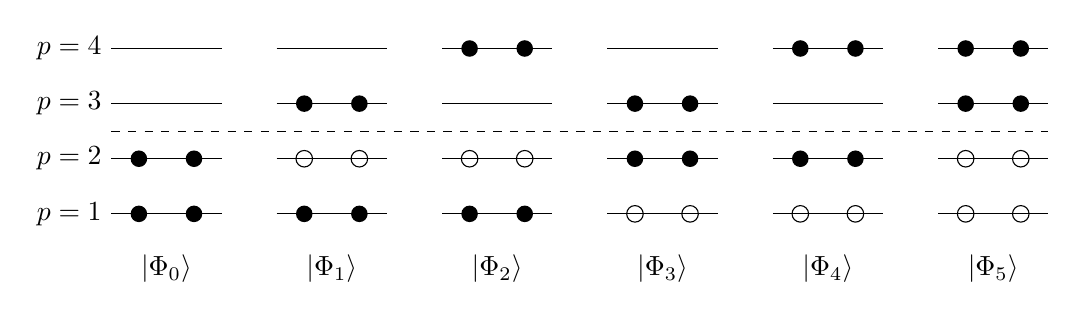
\begin{tikzpicture}[scale=0.7]
    % Draw lines
    \foreach \x in {0,3,6,9,12,15} {
        \foreach \y in {1,2,3,4} {
            \draw (\x, \y) -- (\x+2, \y);
        }
    }
    % Draw additional dashed lines
    \draw[dashed] (0, 2.5) -- (17, 2.5);

    % Labels on the left
    \foreach \y/\label in {1/$p=1$, 2/$p=2$, 3/$p=3$, 4/$p=4$} {
        \node[left] at (0, \y) {\label};
    }

    % Groundstate
    \foreach \x/\y in {0.5/1, 0.5/2, 1.5/1, 1.5/2} {
        \fill (\x, \y) circle (0.15);
    }
    \node at (1, 0) {$|\Phi_0\rangle$};

    % Phi_1
    \foreach \x in {3.5, 4.5} {
        \foreach \y in {1, 3} {
            \fill (\x, \y) circle (0.15);
        }
        \draw (\x, 2) circle (0.15);
    }
    \node at (4, 0) {$|\Phi_1\rangle$};

    % Phi_2
    \foreach \x in {6.5, 7.5} {
        \foreach \y in {1, 4} {
            \fill (\x, \y) circle (0.15);
        }
        \draw (\x, 2) circle (0.15);
    }
    \node at (7, 0) {$|\Phi_2\rangle$};

    % Phi_3
    \foreach \x in {9.5, 10.5} {
        \foreach \y in {2, 3} {
            \fill (\x, \y) circle (0.15);
        }
        \foreach \y in {1} {
            \draw (\x, \y) circle (0.15);
        }
    }
    \node at (10, 0) {$|\Phi_3\rangle$};

    % Phi_4
    \foreach \x in {12.5, 13.5} {
        \foreach \y in {2, 4} {
            \fill (\x, \y) circle (0.15);
        }
        \foreach \y in {1} {
            \draw (\x, \y) circle (0.15);
        }
    }
    \node at (13, 0) {$|\Phi_4\rangle$};

    % Phi_5
    \foreach \x in {15.5, 16.5} {
        \foreach \y in {3, 4} {
            \fill (\x, \y) circle (0.15);
        }
        \foreach \y in {1, 2} {
            \draw (\x, \y) circle (0.15);
        }
    }
    \node at (16, 0) {$|\Phi_5\rangle$};

\end{tikzpicture}
